% REMEMBER: You must not plagiarise anything in your report. Be extremely careful.

\documentclass{l4proj}

    
%
% put any additional packages here
\usepackage{blindtext}
\usepackage{amsmath}
\let\openbox\relax
\usepackage{amsthm}

% theorem environments

\theoremstyle{definition}

\newtheorem{definition}{Definition}[chapter]

\newtheorem{examp}[definition]{Example}

\newenvironment{example}{\begin{examp}}{\hfill$\qed$\end{examp}}


\newcommand{\gethin}[1]{\marginpar{\footnotesize \color{blue} {\bf G:} \textsf{#1}}}

\begin{document}

%==============================================================================
%% METADATA
\title{Modelling and analysis of dice-based stochastic games}
\author{Lewis Dyer}
\date{}

\maketitle

%==============================================================================
%% ABSTRACT
\begin{abstract}
    This project investigates the use of model checking using PRISM to evaluate the game design of various games of chance involving dice. [RESULTS HERE].
\end{abstract}

%==============================================================================

% EDUCATION REUSE CONSENT FORM
% If you consent to your project being shown to future students for educational purposes
% then insert your name and the date below to  sign the education use form that appears in the front of the document. 
% You must explicitly give consent if you wish to do so.
% If you sign, your project may be included in the Hall of Fame if it scores particularly highly.
%
% Please note that you are under no obligation to sign 
% this declaration, but doing so would help future students.
%
%\def\consentname {My Name} % your full name
%\def\consentdate {20 March 2018} % the date you agree
%
\def\consentname {Lewis Dyer}
\def\consentdate {}
\educationalconsent

\chapter*{Acknowledgements}

I would like to express my gratitude to Dr. Gethin Norman, my project supervisor, for his continual support and guidance throughout the project. I would also like to thank William Kavanagh for offering several useful suggestions throughout the project. Finally, I would like to thank my parents for their encouragement and support throughout what has been a rather eventful year.

%==============================================================================
\tableofcontents

%==============================================================================
%% Notes on formatting
%==============================================================================
% The first page, abstract and table of contents are numbered using Roman numerals and are not
% included in the page count. 
%
% From now on pages are numbered
% using Arabic numerals. Therefore, immediately after the first call to \chapter we need the call
% \pagenumbering{arabic} and this should be called once only in the document. 
%
% Do not alter the bibliography style.
%
% The first Chapter should then be on page 1. You are allowed 40 pages for a 40 credit project and 30 pages for a 
% 20 credit report. This includes everything numbered in Arabic numerals (excluding front matter) up
% to but excluding the appendices and bibliography.
%
% You must not alter text size (it is currently 10pt) or alter margins or spacing.
%
%
%==================================================================================================================================
%
% IMPORTANT
% The chapter headings here are **suggestions**. You don't have to follow this model if
% it doesn't fit your project. Every project should have an introduction and conclusion,
% however. 
%
%==================================================================================================================================

\chapter{Introduction}
\label{introduction}

% reset page numbering. Don't remove this!
\pagenumbering{arabic}

In this section, we motivate the importance of game design, explain why model checking is a useful technique for determining game balance, and outline the structure the dissertation.

A key aspect of game design is ascertaining the balance of a game, particularly in reference to different possible strategies for playing the game. As players repeatedly play a game, their aim is to employ better strategies at winning over time, eventually approaching the optimal strategy for a game. However, in practice, the optimal strategy for a game should be complex enough that human players cannot employ this strategy in practice, since a simple optimal strategy leads to a game which is predictable and no longer interesting for players. For instance, the game of Noughts and Crosses has an extremely simple optimal strategy which human players learn almost immediately. Conversely, games such as Chess and Go have optimal strategies, but their complexity makes them infeasible to compute, leading to complex strategic decisions over thousands of years of gameplay.

While these games are entirely based on strategy, many games utilise random elements in order to encourage players to adapt their strategies as the game progresses, making games more interesting and enjoyable to play. One particularly common method for introducing random elements into a game is via the use of dice, which are cheap, satisfying to roll and well understood by the majority of players. Consequently, this dissertation focuses on games which use dice as a key mechanic in the game.

Currently, the most common method of evaluating game balance is via manual \emph{playtesting}, where players repeatedly play early versions of games, providing feedback which designers can use in order to refine their games. However, this method is flawed for multiple reasons. Playtesting is resource intensive, requiring many people to spend significant amounts of time playing a game. In addition, for complex games with many possible actions, playtesting cannot consider all possible strategies. A more subtle issue is that playtesters are often experienced players, who may attempt to apply knowledge from other games in order to play effectively. This further limits the possible strategies that playtesters end up employing. These reasons motivate the use of an automated approach to analysing games, such as probabilistic model checking.

In many systems, simulation and testing are the two primary methods for analysing the behaviour of a system. While these methods are generally simple to implement, a key issue with these methods is that the system is not exhaustively analysed, and in particular statistical methods may fail to accurately consider the probability of rare events occurring in a game. By contrast, probabilistic model checking exhaustively considers all possible actions at each point of a game, leading to more precise observations about a game.

The remainder of the dissertation is outlined as follows. Chapter~\ref{background} discusses preliminary background information for the case studies presented in the dissertation, including an introduction to probabilistic model checking and the PRISM model checker. Chapters~\ref{cs1},~\ref{cs2:liars_dice} and~\ref{ch:cs3} present the case studies, discussing specific examples of games in more detail, including extending models in order to allow for more complex types of games. Chapter~\ref{evaluation} discusses several tools developed in order to improve the rigour of the experiments performed throughout the case studies, while Chapter~\ref{conclusion} summarises the project and offers multiple suggestions for future work.

%==================================================================================================================================


\chapter{Background (3 pages)}

Give context on existing work, both in model checking and in automated game design (RMT coursework very helpful for this). Identify a gap in current work (e.g certain types of games that haven't been analysed very much, or discussion on robustness of models). How can I tie this into my project?

Note: don't go into specific details about model types here (MDPs/POMDPs/CSGs) - leave them to later on.

The very key points I need to mention:

\begin{itemize}
    \item Probabilistic model checking
    \item PRISM specifics
    \item Property specification
    \item Stochastic games
    \item Previous work in automated game balancing
    \item Gap in current work (e.g focus on dice/hidden information/weighted dice?)
\end{itemize}

In order to begin formal analysis of a game, we must first formally define a model of a game, along with properties of this game we wish to consider.

\section{Discrete-time Markov chains}
\label{back:stoc_game}

We first introduce discrete-time Markov chains (or DTMCs), as described by Kwiatkowska et al. in \cite{kwiatkowska_stochastic_2007}. This model is refined and adapted in each case study to develop different types of model suited to different types of games.

\begin{definition}
\label{back:dtmc}
    Given a set of atomic propositions, denoted $AP$, a discrete-time Markov chain (DTMC) is defined as a tuple $\mathcal{D} = (S, \bar{s}, \mathbf{P}, L)$ such that:

    \begin{itemize}
        \item $S$ is the finite set of states;
        \item $\bar{s}$ is the initial state;
        \item $\mathbf{P} : S \times S \rightarrow [0,1]$ is the \emph{transition probability matrix}, where $P(s, s')$ is the probability of transitioning from state $s$ to state $s'$, such that the sum of probabilities of outgoing transitions from each state is $1$.
        \item $L: S \rightarrow 2^{AP}$ is the \emph{labelling function}, where for $s \in S$ a state, $L(s)$ denotes the subset of atomic propositions which hold at that state.
    \end{itemize}

\end{definition}

From this definition of a DTMC, we also define the states where an atomic proposition holds.

\begin{definition}
\label{back:sat}

    For $a \in AP$ and a set of states $S$ as in Definition \ref{back:dtmc}, denote $Sat(a) = \{s \in S \mid a \in L(s)\}$.

\end{definition}


As a motivating example, we define a classic board game using a DTMC.

\begin{example}
\label{back:chess}
    A game of chess can be defined as a DTMC from Definition \ref{back:dtmc} as follows:

    \begin{itemize}
        \item $S$ is the set of states for the game, representing all possible board positions throughout a game of chess, along with the current player's turn (since a given board position could be obtained where either black or white is the current player).
        \item $\bar{s}$ is the initial board position of a standard game of chess, where white makes the first move.
        \item $\mathbf{P}$ assigns each valid move a probability of being chosen at a particular board position. More precisely, a transition to a board position is only valid if the transition can be presented by one legal move according to the rules of chess by the player whose move it is (for instance, the white player can only move white pieces, can only move one piece per move with the exception of castling, and cannot move a piece if the black player can capture the white king in the following turn).
        \item $L$ labels each state with a set of propositions which are true at that state. For instance, if we let $\mathbf{C_w}$ be the atomic proposition that the white player is in check in a given state, then for $s \in S$ a state, $\mathbf{C_w} \in L(s)$ means that the white player is in check in state $s$.
    \end{itemize}

    In this model, the key aspect in determining the skill level of the players is in the transition probability matrix. In theory, there is always an optimal move to make in chess, so for each board position, an optimal player's transition probability matrix will return $1$ for precisely one transition, and return $0$ for all other transitions. But in practice chess is far too complex for players, human or computer alike, to compute this optimal strategy. Hence players choices may be probabilistic, such as a chess player who occasionally "blunders", making a move which places them in a disadvantageous position.
\end{example}

Playing a game is represented as an infinite \emph{path}, denoted as a sequence $\omega = s_0 \rightarrow s_1 \rightarrow \dots$ where $\mathbf{P}(s_k, s_{k+1})>0$ for all $k\geq0$, or in other words where each transition is possible. Note that in states where a game terminates (for instance, states where either the white or black player is in checkmate, or where the game ends in stalemate), we typically define a self-loop in each of these states with probability 1 to ensure the path remains infinite.

DTMCs may also be augmented with \emph{rewards} - numerical values representing various characteristics of a particular execution of a DTMC.

\begin{definition}
\label{back:reward_structure}

A \emph{reward structure} for some DTMC $\mathcal{D}$ is a tuple $(\rho, \iota)$. $\rho : S \rightarrow \mathbb{N}$ is a state reward function, associating each state with the value of a reward, while $\iota : S \times S \rightarrow \mathbb{N}$ is a state transition function, associating each transition with the value of a reward.
\end{definition}

\begin{example}\label{rew:eg}
Returning to Example~\ref{back:chess}, we may define a reward structure $R_w = (\rho_w, \iota_w)$ where $\rho_w$ returns $0$ for all states, and $\iota_w$ returns $1$ for all transitions where the white player captures a black piece.
\end{example}

Note that the reward values may be real-valued (though they may never be negative), but we only consider reward values from $\mathbb{N}$ - Definition~\ref{back:reward_structure} may be modified accordingly to allow for reward values in $\mathbb{R}_{\geq0}$. These reward values can be utilised and examined in various different ways to evaluate a DTMC. More detail on this is provided in Section~\ref{back:prop_spec}, but in particular the expected value of a reward value over all possible paths through a DTMC is frequently considered during model checking.


\section{Property specification}
\label{back:prop_spec}

When analysing probabilistic models, including DTMCs, we consider two main types of properties: \emph{probabilistic reachability} properties and \emph{reward-based} properties. We may define properties in terms of \emph{Probabilistic Computation Tree Logic} (PCTL), as defined by Hansson and Jonsson~\cite{hansson_logic_1994}. These properties are comprised of path quantifiers and temporal operators, though for the purposes of this dissertation we only consider one temporal operator. In particular, the future operator, denoted $\mathbf{F}$, considers whether a particular proposition \emph{eventually} holds for some state on a given path.

A closely related operator is the until operator, denoted  $\mathbf{U}$, which considers two propositions, say $a$ and $b$, and determines whether for a given path, $a$ always holds before some state, then $b$ holds for the given state. Indeed, the future operator is actually equivalent to the until operator when $a$ is the proposition which always holds, denoted \verb+true+. We use this equivalence in Section~\ref{back:prob_mod_check} in order to perform model checking on probabilistic reachability properties.

For probabilistic reachability properties, we also include the $\mathbf{P}$ operator, which considers the probability of a particular property holding across all possible executions of the DTMC. For instance, using Example \ref{back:chess}, if we define $\mathtt{white\_win}$ as the proposition that white is considered to have won the game in the current state, the property $\mathbf{P}_{=?} [\mathbf{F}\ \mathtt{white\_wins}]$ represents the probability that white eventually wins the game of chess. We may similarly define bounded properties in a similar manner, such as $\mathbf{P}_{\geq 0.5} [\mathbf{F}\ \mathtt{white\_wins}]$, denoting whether or not white eventually wins with probability greater than $0.5$, although we introduce bounded properties solely to introduce notation, and do not formally consider model checking bounded properties.

For reward-based properties, PRISM defines an extension to PCTL introducing the $\mathbf{R}$ operator~\cite{kwiatkowska_stochastic_2007}, which allows for properties where the value of a reward is taken into account. For the purposes of this dissertation we only consider one type of reward-based property, namely the \emph{reachability reward} property, referring to the expected cumulative value of a reward along a path, until a state satisfying a particular proposition is reached.

\begin{example}
\label{back:chess_reward}
Again building on Example \ref{back:chess} and using the reward structure from Example~\ref{rew:eg}, the property $\mathbf{R}_{=?} [\mathbf{F}\ \mathtt{white\_win}]$ represents the expected value of the difference between the number of pieces the white and black player control in the cases where the white player eventually wins. 
\end{example}

These reward-based properties can provide useful information when balancing games. For instance, we may initially expect that the difference in pieces captured is a useful measure of how "close" a game of chess is, and this measure could be evaluated via model checking, where we may find it insufficient as a balance measure. For instance, this measure gives equal weighting to every piece, whereas some pieces such as queens are often considered more valuable than other pieces. This behaviour can be modified by changing the state transition function of the reward structure from Example \ref{back:check_rewards}, such as by defining $\iota_w$ such that it returns $1$ when the white player captures a black pawn, and $\iota_w$ returns $2$ when the white player captures a black piece that is not a pawn.
\section{Probabilistic model checking}
\label{back:prob_mod_check}

% This is good, but definitely more like introduction/motivation

%As we have established, many games exhibit probabilistic behaviour. For instance, board games frequently make use of dice in order to introduce random elements into a game, in order to improve the game's replayability. Moreover, the strategies employed while playing these games are often probabilistic. For instance, games with a high degree of non-transitivity encourage probabilistic strategies, since the lack of optimal action means that non-probabilistic strategies are relatively simple to exploit. To give an example, in the game of rock paper scissors, the strategy of always playing scissors will always lose against the strategy of always playing rock.

%As a result of this, typical verification techniques relying on random samples, such as Monte Carlo methods, can be unreliable when considering properties of stochastic games. Statistical methods can only ever provide \emph{probabilistic} guarantees about the game, since the series of samples taken may be entirely unrepresentative of typical gameplay. Moreover, when considering the optimal behaviour of a game, we frequently encounter cases of nondeterminism, where a choice must be made. Most statistical techniques currently resolve nondeterminism uniformly, which amounts to making choices at random, without any particular rationale or analysis behind these choices. Hence we require a more sophisticated class of techniques for analysing stochastic games.


Now that we have defined a DTMC, along with properties of that DTMC to consider, we now define probabilistic model checking - the class of methods for verifying the probability of some event occurring during the process of playing a game. Compared to non-probabilistic model checking, this presents some unique challenges, such as in the following example.

\begin{example}
\label{back:chess-reachability}
    Consider a game of chess, defined in Example \ref{back:chess}, let $\mathbf{M_w}$ and $\mathbf{M_b}$ be the atomic propositions that the white player and black player, respectively, are in checkmate in a particular position. In non-probabilistic model checking, we may consider the reachability of $\mathbf{M_w}$ - in other words, we consider whether we can always reach a state where the white player is in checkmate, regardless of which reachable board position we start in.
    
    In particular this result is binary - either we can always reach a state where $\mathbf{M_w}$ holds, or there exists a board position where white can never lose via checkmate. Indeed, in chess the latter holds - for instance, if the black player only has a king remaining, then there is no way for white to lose via checkmate, since black has insufficient material. And since our model is essentially a directed graph, we can employ standard widely-known algorithms such as a breadth first search in order to verify such reachability properties.

    However, if we consider probabilistic model checking, then as well as qualitative properties, such as the above, we can also consider quantitative properties, such as the \emph{probability} that the white player is in checkmate from a particular board position. In PCTL, this may be expressed as the property $\mathbf{P}_{=?} [\mathbf{F} \, \mathbf{M_w}]$. This is a far more general and powerful property - for instance, an advanced chess player, who has found themselves in a state such that they are in disadvantage over the other player, may seek to reach states where the game is unlikely to end in checkmate, maximising the probability of a draw. However calculating this probability is more complex than for non-probabilistic reachability problems, since we must also consider every possible path that can be taken in order to reach a particular state.
\end{example}

As we defined reachability and reward-based properties separately, we also define model checking reachability and reward-based properties separately, although the methods used in each type of property are similar.

\subsection{Model checking probabilistic reachability properties}
\label{back:check-reach}

Evaluating probabilistic reachability properties is a recursive process, since we need to consider the probabilistic reachability of each state that a given state can reach. Hence we need to define the "base cases" of this recursion, which are described below as in \cite{kwiatkowska_stochastic_2007}, with slightly different notation.

\begin{definition}
\label{back:S_yes}

    For a DTMC $\mathcal{D}$, with a set of states $S$ and a given atomic proposition $a$, we can partition the state space into three subsets as so:

    \begin{itemize}
        
        \item $S^{yes}$ is the set of all states where $a$ eventually holds with probability 1.
        \item $S^{no}$ is the set of all states where $a$ never holds in any subsequent reachable state.
        \item $S^{?} = S \setminus (S_{yes} \cup S_{no})$ the set of all states where the probability of $a$ holding eventually is in the interval $(0,1)$.

    \end{itemize}

\end{definition}

The sets $S^{yes}$ and $S^{no}$ are fairly straightforward to compute using graph-based algorithms. The precise details of their construction are described further in \cite{kwiatkowska_stochastic_2007}, but $S^{no}$ is constructed via a simple reverse traversal of the DTMC, starting from $Sat(a)$ and obtaining all states that can reach a state in $Sat(a)$, then removing these states from $S$. $S^{yes}$ is constructed very similarly, except this construction starts with $S^{no}$ and traverses the DTMC to find all states where the probability of reaching a state in $Sat{a}$ is less than 1, then removing these states from $S$.

After this precomputation process, we can now calculate the probability of a probabilistic reachability property holding over the entire state space $S$, by extending the probability calculation over the states in $S^{?}$.

\begin{definition}
\label{back:F_operator}

    For a DTMC $\mathcal{D}$, with a set of states $S$, a partition of $S$ as in Definition \ref{back:S_yes}, and an atomic proposition $a$, we denote $Prob^{\mathcal{D}}(s, \mathbf{F} \: a)$ as the probability that an execution of $\mathcal{D}$ starting at state $s$ eventually reaches a state where $a$ holds. Furthermore, we have for any $s \in S^{?}$ that:

    \begin{equation*}
        Prob^{\mathcal{D}}(s, \mathbf{F} \: \Phi) = \sum_{s' \in S^{?}} \mathbf{P}(s, s') \cdot Prob^{\mathcal{D}}(s, \mathbf{F} \: \Phi) \: + \sum_{s' \in S^{yes}} \mathbf{P}(s, s')
    \end{equation*}
    
\end{definition}

From Definition \ref{back:F_operator}, calculating reachability probabilities requires solving a system of linear equations containing $|S^{?}|$ unknowns. There are many different methods for solving these equations, but in practice iterative methods (such as the Gauss-Siedel method or power iteration) are preferred to direct methods (such as Gaussian elimination) - iterative methods generally do not give exact solutions, opting for values which eventually converge to an exact solution, but direct methods can require more time and space to compute an exact solution, and in many circumstances the performance improvements justify a slightly less precise result.

\subsection{Model checking reward-based properties}
\label{back:check_rewards}

The approach to model checking reward-based properties is similar in spirit to checking reachability properties, in that we recursively construct a series of linear equations, which may be solved using any standard method. However, a key remark is that, when evaluating the expected cumulative reward value until a state where some proposition $a$ holds, we assume that a state where $a$ holds is always eventually reached with probability 1. If this does not occur for some path in a DTMC, then a reward can accumulate infinitely often. Hence, the expected reward value in this case is considered to be infinite.

In order to evaluate reward-based properties, we first define a random variable representing the cumulative reward value of an arbitrary infinite path.

\begin{definition}
\label{back:reach_reward}

For a DTMC $\mathcal{D}$, let $Path(s)$ be the set of all paths of $\mathcal{D}$, starting in some stats $s$, and let $T$ be the set of states in $\mathcal{D}$ where some proposition $a$ holds, along with denoting $\rho$ and $\iota$ as state and transition reward functions respectively. Then $X_{Reach(T)} : Path(s) \rightarrow \mathbb{R}_{\geq 0}$ is a random variable where, for any infinite path $\omega = s_{0} s_{1} s_{2} \dots$:

    \begin{equation*} 
        X_{Reach(T)}(\omega) = 
            \begin{cases}
                0 & s_0 \in T \\
                \infty & \forall i \geq 0 . \, s_i \notin T  \\
                \sum_{i=0}^{k_{T} - 1} \rho(s_i) + \iota(s_i, s_{i+1}) & \text{otherwise}
            \end{cases}
    \end{equation*}

where $k_T = min \{ j \mid s_j \in T \}$, the first state in the path where the atomic proposition $a$ holds.

From this, we then define $ExpReach(s, T) = \mathbb{E}(X_{Reach(T)})$, the expected value of the cumulative reward value over all possible infinite paths through $\mathcal{D}$, starting from state $s$.

\end{definition}

Model checking reward-based properties consists precisely of calculating $ExpReach(s, T)$ for all $s \in S$,  which can be expressed as the solution of a system of linear equations using the above definition:

\begin{equation*}
    ExpReach(s, T) = 
        \begin{cases}
            \infty & s \in Sat(\mathbf{P}_{<1} [\mathbf{F} \; a]) \\ 
            0 & s \in T \\
            \rho(s_i) + \sum_{s' \in S} \mathbf{P}(s, s') \cdot \left( \iota(s_i, s_{i+1}) + ExpReach(s', T) \right) & \text{otherwise}
        \end{cases}
\end{equation*}

Note that $ExpReach(s, T) = \infty$ precisely where there exists some path in $Path(s)$ such that $a$ never eventually holds, or equivalently where $T$ is never reached.

\section{The PRISM model checker}
\label{back:PRISM}

PRISM \cite{kwiatkowska_prism_2011} is a software tool which implements probabilistic model checking on a wide variety of models. In particular, PRISM defines two languages in order to facilitate model checking: the \emph{PRISM language} for formally defining models, along with the \emph{PRISM property specification language} for formally defining PCTL properties (or rather, an extension of PCTL adding reward-based properties).

\subsection{The PRISM modelling language}
\label{back:PRISM-modelling}

PRISM provides a modelling language in order to formally specify probabilistic models. In particular, many probabilistic models exhibit \emph{emergent complexity}, where simple descriptions of behaviour can lead to complex models. Hence, a modelling language is essential to allow describing the behaviour of a model, rather than a more complicated model specification. Note that we do not provide a full description of the PRISM modelling language here, instead focusing on the key features used in the various case studies - more details are available in the PRISM manual \cite{noauthor_prism_nodate}, along with additional examples.

PRISM models are defined as a set of \emph{modules}, where each module consists of a set of \emph{variables} and a set of \emph{commands}. Variables may be either integers or boolean values, and in particular integers must be bounded, since otherwise the state space of a model is unbounded. Variables can be accessed by any module, but modules can only alter their own variables.

The key structure of a PRISM model is a \emph{command}, of the following form:

\begin{verbatim}
    [] guard -> prob_1 : update_1 + ... + prob_n : update_n;
\end{verbatim}

A \emph{guard} represents a proposition, identifying the set of states where the command is applicable. The command here has $n$ transitions, with a probability of each transition occurring such that the probabilities sum to $1$. Each update is comprised of a set of variable updates. And each possible combination of values for each variable represents a state of the resulting model, so a set of variable updates represents a transition between two states.

Note that guards may overlap, including between modules. This behaviour is handled differently depending on the type of model being constructed. For a DTMC each command which is enabled has an equal probability of being selected, but for other model types overlapping guards induce nondeterministic choice - a key aspect of defining strategies for games, as described further in the case studies.

In some cases, there may be a desire for modules to synchronise commands - for instance, two players making a decision simultaneously. This behaviour is supported via the use of \emph{action labels}. As an example, consider the following PRISM command:

\begin{verbatim}
    [cover_1] b1=0 -> (b1'=1);
\end{verbatim}

Here, very little logic is given for when the variable \verb+b1+ is updated. However, the \verb+cover_1+ action label allows this command to synchronise with another command with the same action label in another module. This is especially useful for defining "updater" modules - modules which control a particular variable and perform updates, but make no contribution towards the decision making of a particular model. We also note that action labels may be used even where no explicit synchronisation takes place. Indeed, action labels are frequently used in order to describe an execution of a model, which is particularly useful when debugging a model via manual simulation.

For convenience, PRISM models also define \emph{formulas} and \emph{labels}. Formulas act as shorthand for a particular expression, allowing for a complex expressed to be referred to on multiple occasions without needless code duplication. A simple example of a formula is given below:

\begin{verbatim}
    formula score = b1*1 + b2*2 + b3*3 + b4*4 + b5*5 + b6*6;
\end{verbatim}

Labels serve a very similar purpose, but they are boolean expressions which define a set of states satisfying a particular proposition, which are frequently used when specifying properties. For instance, the following label shows how labels can be utilised to define a particular characteristic of states of a model:

\begin{verbatim}
    label "game_over" = (phase>=6);
\end{verbatim}




Finally, PRISM allows for specifying reward structures. Reward structures comprise of a guard specifying when the reward is applicable, along with the value of a reward when this guard is satisfied. Note that PRISM supports two main types of rewards - instantaneous rewards, considering the value of a reward in a specific state, and cumulative rewards considering the total value of a reward throughout an execution of the model.  The following example represents a reward which is intended to be cumulative:

\begin{verbatim}
    rewards "no_rolls"
        state=0: 1;
    endrewards
\end{verbatim}

Alternatively, the following reward is intended to be instantaneous, representing the number of cards in a player's hand, which may change throughout the course of some game:

\begin{verbatim}
    rewards "cards_in_hand"
        true: card_count;
    endrewards
\end{verbatim}

Note that this distinction between cumulative and instantaneous rewards is purely contextual, and hence the correct reward type to use is based on the intended behaviour of the reward, as opposed to any inherent characteristics of the reward itself. Hence, this distinction is applied at the property specification stage, rather than model construction.

Action labels may also be utilised in order to represent transition rewards, such as the following example counting the number of times a player chooses to roll 2 dice:

\begin{verbatim}
    rewards "2_rolls"
        [roll_2_dice] true : 1
    endrewards
\end{verbatim}




\subsection{The PRISM property specification language}
\label{back:PRISM-prop}

When specifying properties of a model to be evaluated, PRISM defines a property specification language which supports and extends a variety of probabilistic temporal logics, although for the purposes of this dissertation we only consider the extension of PCTL with reward-based properties, as described in \ref{back:prop_spec}. As a simple example, consider the following property in PRISM:

\begin{verbatim}
    P=? [ F game_over&score=10 ]
\end{verbatim}

The main difference between the PRISM modelling language and "pure" PCTL syntax is the definition of the atomic proposition. Here, we refer to labels and variables from within a PRISM module in order to define an atomic proposition, allowing us to easily define a set of states where this proposition holds, namely where the game is over and the current score is 10. Reward-based properties can also be defined in a similar manner:

\begin{verbatim}
    R{"total_boards"}=? [ F game_over ]
\end{verbatim}

Note that PRISM models may contain many possible reward structures, so we specify the particular reward structure considered here using braces.

The PRISM modelling language provides a convenient way to express properties in PCTL, but one particular syntactic benefit of the PRISM modelling language is the use of undefined constants. For instance, consider adapting the above probabilistic reachability property in order to use an undefined constant for the score:

\begin{verbatim}
    const int k;
    P=? [ F game_over&score=k ]
\end{verbatim}

When model checking is performed, an \emph{experiment} can be defined, where different values of \verb+k+ may be considered. For instance, if the value of \verb+score+ is bounded, then allowing \verb+k+ to vary over all possible values of \verb+score+ can be utilised in order to produce a probability distribution of \verb+score+ when the model terminates.

%% move this to games section later on
% In addition, later on in the case studies, we define nondeterministic models, along with coalitions. Hence, properties may look more similar to this:
% 
% \begin{verbatim}
%     <<p1>>Pmax=? [ F game_over&score=k ]
% \end{verbatim}
% 
% In this property, \verb+<<p1>>+ denotes the set of players in the \emph{coalition} - in other words, players whose actions may be directly controlled. Moreover, \verb+Pmax+ means that the maximum probability is considered \emph{under all possible resolutions of nondeterminism}. In particular, care must be taken when computing conditional probabilities, since in general the decisions made in order to obtain the lower bound and the upper bounds of a particular probability are rather different. 

\section{Related work}

% just copying over RMT for now, will probably edit a fair bit

\label{back:related}

One of the first papers to discuss automatic game balancing was presented by Hom and Marks \cite{hom_automatic_2007}, who focused on combining and mutating the rules of various classic board games using genetic algorithms in order to define a new game, whose win rate was then analysed using a commercial game engine to determine the game's balance. A key feature of future work in automatic game balancing is the development of more sophisticated measures of balance. Hom and Marks primarily focused on two-player games using the win rate of each player, while Jaffe et al. \cite{jaffe_evaluating_2012} built on this foundation by developing a framework designed around answering a wider variety of balance questions, such as the importance of short-term and long-term strategy in decision making, via the use of "restricted players" - optimal AI agents with specific restrictions on how they make decisions, such as being unable to consider the opponent's actions for several rounds at the beginning of a game, facing optimal opponents who are able to exploit these restrictions.

These ideas are then applied by Milazzo et al. \cite{milazzo_case_2015}, using probabilistic and statistical model checking in multiple case studies to answer balance questions about games. In particular, the authors show that model checking can be applied to balance games on several different "levels" at once, both adjusting the parameters of various game mechanics and the inclusion of these mechanics in the first place (such as adjusting how much health players have, whether players can have multiple lives, and how these mechanics interact). This idea is further extended to develop Chained Strategy Generation \cite{kavanagh_balancing_2019}, a technique for balancing games over the course of a \emph{metagame}, where different selections of material choice in a game (such as players or teams in a football game) change in popularity over time. Kavanagh and Miller also consider an alternative formulation of player skill in \cite{kavanagh_gameplay_2020}, where actions have an associated \emph{cost} based on comparison with the best possible action in a particular state.

However, this literature review revealed a significant gap in current research on formal verification in game balancing. The games which have currently been considered are primarily turn-based, and more crucially they are all \emph{perfect information} games, where the current state of the game is fully visible to all players. As a result, a key aim of this dissertation is to consider model checking on a wider variety of games.

Throughout the case studies in this dissertation, the first is designed to be fairly conventional relative to existing literature on analysing games via model checking. The second and third case studies consider hidden information games and concurrent games respectively, which we do not believe have been considered in previous literature.


%==================================================================================================================================

\chapter{Case Study 1: Shut the Box}


\section{Game description (1/2 page)}
Describe the game, mention some variants, set out the sorts of questions we'd like to answer about the game.

\hrule

\blindtext

\blindtext

\blindtext

\section{Background (1 page)}

Describe MDPs here, explain why they're a suitable tool to model Shut The Box (essentially a 1 player game).

\hrule

\Blindtext

\section{Analysis (3 pages)}

Collect some data, show the results.

\hrule

\Blindtext

\Blindtext

\Blindtext

\section{Evaluation(2 pages)}

The key section - use the results from model checking to answer questions about the game (for instance, to examine the difficulty and/or complexity of a game).

\hrule

\Blindtext

\Blindtext

%==================================================================================================================================

%\chapter{Case Study 2 (Liar's Dice)}

In this case study, we introduce Liar's Dice, a dice game utilising hidden information. We introduce partially observable MDPs (known as POMDPs) to represent this hidden information, model a small version of the game using a POMDP, and analyse the susceptibility of Liar's Dice to the snowball effect.

\section{Liar's Dice description}
Liar's Dice is a dice game for multiple players, where each player must be able to bluff and detect opponent's bluffs in order to win. Liar's Dice takes place over a series of rounds, where each player rolls their dice, keeping the values on the dice hidden from other players. A player then makes a \emph{bid}, which is comprised of a face value ono a dice, and the number of dice that show that value. Players then rotate in turn, choosing to either make a higher bid (with either a higher face value, a higher quantity, or both), or challenge the previous bid. If a challenge is made, all dice are revealed. If the bid was correct, the challenging player loses a die. If the bid was incorrect, the bidding player loses a die. The player who lost starts the next round, and play continues until only one player has any remaining dice.

In Liar's Dice, every player starts with the same amount of information, since every player starts with the same number of dice. However, as the game progresses, some players will have more dice than others, changing bidding behaviour, as demonstrated by the following example:

\begin{example}
\label{cs2:hidden_info_example}

Consider the situation presented in Figure \ref{cs2:uneven_information}, where the first player has rolled two 2s while the second player has rolled a 5. The first player can confidently make a bid that there are two 2s, but the second player cannot see enough dice to determine the correctness of this bid. Hence, the second player has three options:

\begin{itemize}

\item If the second player challenges the bid, they will lose a dice, and therefore lose the game.
\item If the second player increases the face value of the bid, then the first player can immediately challenge the bid and win the game, since they know that at most one dice cannot have value 2.
\item If the second player increases the quantity of the bid, to bidding that there are three 2s, the first player can challenge and win with probability $\frac{5}{6}$.

\end{itemize}

As a result, the first player is able to use their increased access to information in order to increase their chances of success.

\end{example}

\begin{figure}[h]
    \centering
    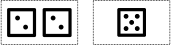
\includegraphics[width=0.7\textwidth]{images/LiarsDice/different_information.pdf}
    \caption{A game of Liar's Dice, where the first player has rolled two 2s while the second player has rolled a 5.}
    \label{cs2:uneven_information}
\end{figure}

This example represents a potential issue with the design of Liar's Dice. Initially we expect that the probability of either player losing a round is even, depending primarily on the strategies the players employ. However, as the game progresses, players with fewer dice are more likely to lose subsequent rounds, making it harder and harder for players to win from behind, a phenomenon known as the \emph{snowball effect} in game design. 

In particular, the snowball effect means that the overall results of games may be decided fairly early on, even if the games are long. This is frustrating for players - the players are still required to play several rounds of a game where the result is already a foregone conclusion. Moreover, with multiple players, this presents an opportunity for one player to be eliminated very early, since the game continues without their involvement.

Our aim when analysing Shut the Box will be to examine to what extent Liar's Dice exhibits the snowball effect, and whether this effect can be mitigated in some way. Firstly, we introduce a variant of MDPs which allows for partial observability, in order to model the hidden information present in Liar's Dice.

\section{Background (1 page)}

A key aspect of Liar's Dice is partial observability, which we now introduce in order to augment our existing MDPs, as described in \cite{norman_verification_2017}.

\begin{definition}
    \label{cs2:def-pomdps}

    A partially observable Markov decision process (or POMDP) is a tuple $\mathcal{P} = (S, \bar{s}, A, \delta, L, \mathcal{O}, obs)$ such that:

    \begin{itemize}
        \item $(S, \bar{s}, A, \delta, L)$ is an MDP, as in Definition \ref{cs1:def_mdps}.
        \item $\mathcal{O}$ is a finite set of \emph{observations}
        \item $obs : S \rightarrow 2^{\mathcal{O}}$ labels each state with a subset of observations.
        \item For any two states $s, s' \in S$, if $obs(s) = obs(s')$ then the available actions at $s$ and $s'$ must be identical. When this occurs, we say that states $s$ and $s'$ are \emph{observationally equivalent}
    \end{itemize}
\end{definition}

The last point in this definition indicates how POMDPs can represent hidden information. Rather than being able to directly access every state, decisions can only be made based on observations. For instance, in many card games, some cards may be visible for a particular player, while others are hidden. In order for two states to be observationally equivalent in a model of this game, we only require that the visible cards are the same in both states, while the hidden cards can range across any permutation of valid cards.

Since POMDPs are an extension of an MDP, adversaries for POMDPs are defined in terms of adversaries for the corresponding MDP. However, in order to reflect the added constraints that observations provide, we require that adversaries on observationally equivalent paths are equivalent:

\begin{definition}
\label{cs1:pomdp_strats}

For a POMDP $P$, an adversary of $P$ is a function $\sigma$ mapping all finite paths through the POMDP to a discrete probability distribution over the set of actions. In particular, $\sigma$ is also an adversary of the corresponding MDP. Moreover, for paths $\pi = s_0 \xrightarrow{a_0} s_1 \xrightarrow{a_1} \dots s_n$ and $\pi = s'_0 \xrightarrow{a'_0} s'_1 \xrightarrow{a'_1} \dots s'_n$, if $obs(s_i) = obs(s'_i)$ and $a_i = a'_i$ for all $i \in \mathbb{N}$, then $\sigma(\pi) = \sigma(\pi')$. In other words, $\sigma$ makes the same decisions in observationally equivalent paths.

\end{definition}

This definition references a key difference in optimal adversary generation between MDPs and POMDPs. In MDPs, optimal adversaries are deterministic and memoryless, so in particular adversaries map states to actions. This allows for aforementioned methods such as value iteration to be applied, allowing for efficient computation of optimal values and adversaries attaining these optimal values.





Describe POMDPs here - what makes them important and useful compared to MDPs? Explain why we add this additional complexity, but also mention trade offs in terms of the sorts of analysis we can perform.


\section{Analysis (3 pages)}

Collect data, show results. Make sure to mention how game trees are constructed to infer results about games based on individual rounds.


\section{Evaluation (2 pages)}

Again, use model checking results to answer questions about Liar's Dice. Discuss potential limitations of analysis that arise from using POMDPs.



%==================================================================================================================================

%\chapter{Case Study 3 (26.2)}
\label{ch:cs3}

In this section we introduce 26.2, a dice game where players make decisions simultaneously. A new model type is developed in order to facilitate this behaviour, and analyse 26.2 in order to... 

\section{Game description (1/2 page)}

The game of 26.2 takes place over a series of rounds, where players choose how many dice they wish to roll, up to a maximum of ten dice. These dice are all rolled simultaneously, and their values are examined. If three or more of a player's dice have the same face value, or two pairs of two dice have the same face value, the player is said to have \emph{gone bust}, and does not move this round. Otherwise, the player moves forward a number of spaces equal to the sum of each of their dice. When a player reaches space 262 or later, the game ends, and the winner is the player who has travelled the furthest. If this results in a tie, a winner is randomly selected from the players who have tied.

One key aspect of this game is that players simultaneously choose how many dice they roll. This allows for some interesting decision making, as discussed in the following example:

\begin{example}
\label{cs3:example_concurrency}

In a game of 26.2, suppose that player 1 and player 2 are both 5 spaces away from the goal. Broadly speaking, both players have two options - They can either roll a small number of dice, giving a low probability of going bust, or roll a large number dice, leading to a higher probability of going bust, but also moving more spaces. If 26.2 was not a concurrent game, then player 1 would choose how many dice to roll first, followed by player 2. If player 1 choose to roll a small number of dice, then player 2 could roll a slightly higher number of dice, since this would increase the probability of rolling more spaces than player 1, without substantially increasing the probability of going bust. However, if player 1 instead rolled a high number of dice, then player 2 could roll a small number of dice, anticipating that player 1 has a high probability of going bust.

However, concurrency means that these decisions are made simultaneously, meaning player 2 would have to anticipate how many dice player 1 is going to roll, and make decisions accordingly.

\end{example}

In order to allow for concurrent decision making to be modelled, we need to introduce a new type of model.

\section{Background}

\subsection{Concurrent stochastic games}

As discussed in Example \ref{cs3:example_concurrency}, the addition of concurrency in 26.2 can alter the strategies players adopt. In order to account for this behaviour, we introduce models known as \emph{concurrent stochastic games}, as described in \cite{kwiatkowska_automated_2018}.

\begin{definition}
    \label{cs3:def_csgs}

    A concurrent stochastic game (CSG) is a tuple $\mathcal{G} = (N, S, \bar{s}, A, Act, \delta, AP, L)$ such that:

    \begin{itemize}
        \item $N = \{ 1, \dots, n \} $ is a finite set of players;
        \item $S$ is a finite set of states;
        \item $\bar{s}$ is the initial state;
        \item $A = \left(A_1 \cup \{\perp\} \right) \times \dots \times \left(A_n \cup \{\perp \} \right)$ is the set of actions, where $A_i$ is a finite set of actions available to some player $i$, and $\perp$ represents an idle action which is disjoint from the actions of all other players.
        \item $Act: S \rightarrow 2^{\cup_{i=1}^{n} A_{i}}$ is an action assignment function, where $Act(S)$ denotes the available combinations of actions across all players. In particular, some combinations of actions may be unavailable, even if the individual actions may be available for different players.
        \item $\delta : S \times A \rightarrow Dist(S)$ is a partial transition function.
        \item $AP$ is a set of atomic propositions where $L : S \rightarrow 2^{AP}$ labels each state with a subset of atomic propositions holding at that state.
    \end{itemize}
\end{definition}

This definition has a lot in common with Definition \ref{cs3:def_csgs} - the main difference is that players simultaneously choose actions, and the transition between states depends on the combination of actions chosen by all players. Indeed, an MDP can be considered as a subset of CSGs, specifically where for any state $s$, $A_i \neq \{ \perp \} $ for precisely one player $i$.

We also slightly adapt our definition of paths to accommodate this difference in action selection.

\begin{definition}
    \label{cs3:csgs_paths}

    Given a CSG $\mathcal{G}$, a path $\pi$ is a sequence $s_0 \xrightarrow{\alpha_0} s_1 \xrightarrow{\alpha_1} \dots$, with $s_i \in S$ and $\alpha_i = (a^{i}_1, \dots, a^{i}_n) \in A$, $a^{i}_j \in A_{j}(s_i)$ for $j \in N$, and that $\delta(s_i, \alpha_i )(s_{i+1}) > 0$ for all $i$. A finite path is a truncation of an infinite path.
\end{definition}

And as in the previous case studies, adversaries are defined very similarly, though we must consider adversaries for all players at once.

\begin{definition}
    \label{cs3:csgs_strats}

    For a CSG $\mathcal{G}$, a strategy profile $\sigma$ is a tuple $(\sigma_1, \dots, \sigma_n)$ of strategies for each player. A strategy $\sigma_i$ for some player $i$ maps each finite path $\pi$ to $Dist(A_i)$, such that if $\sigma_i(\pi)(a_i) > 0$, then $a_i$ is an available action for player $i$ at the last state of $\pi$.

\end{definition}

We can also augment CSGs with reward structures as with previous model types, with action rewards and state rewards.

We now introduce methods for computing reachability probablities and reward-based properties in CSGs. These methods are somewhat similar in spirit to those for DTMCs and MDPs, but the computation of specific values requires a new class of techniques.

\subsection{Normal form games and matrix games}
\label{cs3:prop_ver_csgs}

We first discuss some preliminaries from game theory, specifically the idea of matrix games. We start by introducing a simplifed game, known as a \emph{normal form game}.

\begin{definition}
\label{cs3:normal_form_games}

A normal form game $\mathcal{N}$ is a tuple $(N, A, u)$, where $N$ and $A$ are defined as in CSGS in Definition \ref{cs3:def_csgs}, and $u$ is a tuple $(u_i, \dots, u_n)$ where, for a given action $a \in A$, $u_i(a)$ assigns player $i$ a real number, which is the player's utility for the game.

\end{definition}

This game is simpler than the games we have considered in these case studies, since only one action is taken before the end of the game. In addition we only consider two-player zero sum games, which are games where the sum of utilities for each player sum to 0. This allows us to model games with one winner and one loser, by setting a player's utility to $-1$ if they lose and $1$ if they win. This also allows us to express the probability of a player eventually winning from a given position in a game. Given a win probability $p$, the corresponding utility is given by $2p - 1$.

These games may also be represented as a matrix, as shown in the following definition.

\begin{definition}
    \label{cs3:matrix_games}

    Given a two-player zero game normal form game $\mathcal{N}$, the corresponding \emph{matrix game} $Z$ is the $l \times m$ matrix such that $A_1 = {a_1, \dots, a_l}$ and  $A_2 = {b_1, \dots, b_m}$ with $Z_{i, j} = u_{1}(a_i, b_j) = -u_{2}(a_i, b_j)$.
\end{definition}

We are interested in obtaining the \emph{value} of a matrix game, which represents the minimum total value a player can obtain from a game. More specifically, we say that for some matrix game $Z$, $val(Z) = v^*$ if player 1 has an optimal strategy such that the utility of the game is always at least $v^*$, and conversely if player 2 has an optimal strategy such that the utility of the game is at least $-v^*$. Every matrix game has a value, a consequence of the minimax theorem proved by von Neumann in \cite{v_neumann_zur_1928}. This value can be obtained as the solution to a linear programming problem, specifically maximising v subject to the following constraints:

\begin{align*}
v \leq p_1 \cdot Z_{1, j} + \dots + p_l \cdot Z_{l, j} \quad \text{for} 1 \leq j \leq m \\
p_i \geq 0 \: \forall i, \quad p_1 + \dots + p_l = 1
\end{align*}

The solution $(p_1, \dots, p_l)$ yields an optimal strategy for player 1, and the analogous problem for player 2, which involves minimising v, yields an optimal strategy for player 2.

We are now ready to compute reachability probabilities and reward-based properties for CSGs.

\subsection{Property verification for CSGs}
\label{cs3:prop_ver_csgs}

We use a similar approach to Section \label{cs1:prob_reach_mdps} in order to compute $P^{s}[ \; F a]$, where $s$ is some state and $a$ is an atomic proposition, denoting the probability of eventually reaching some state where $a$ holds starting from $s$. Specifically, we define a sequence $(x_s^{n})_{n \in \mathbb{N}}$ denoting the probability of eventually reaching a state where $a$ holds within at most $n$ steps, then use a large enough value of $n$ to converge to the actual probability.

\begin{definition}
    \label{cs1:val_iter_csgs}

    Given a CSG $\mathcal{G}$, we have that:

    \begin{equation*}
    x_s^{n} =
    \begin{cases}
    1 & s \in Sat(a) \\
    0 & s \notin Sat(a), n=0 \\
    val(Z) & \text{otherwise} \\
    \end{cases}
    \end{equation*}

    Specifically, $Z$ is the matrix game with:

    \begin{equation*}
        Z_{i,j} = \sum_{s' \in S} \delta(s, (a_{i}, b_{j}))(s') \cdot x_{s'}^{n-1}
    \end{equation*}

\end{definition}

Computation of reward-based properties is analogous. An important point about the above definition is that CSGs are more involved than normal form games - in particular, CSGs require a sequence of actions whereas normal form games are completed after one action, but we can use a sequence of normal form games to reason about CSGs. Another key aspect of this definition is that the players in a CSG are split into two main "groups", or \emph{coalitions}, with one group aiming to reach the set of target states and one group aiming to avoid the target states. Coalitions are not considered in more depth due to the impact of adding additional players on model size, but they allow for cooperation to be modelled in CSGs.

We now focus on 26.2 in more detail, comparing pre-defined strategies to more complex optimal strategies.

\section{Results and analysis}

To begin with, we discuss a few constraints required to feasibly model 26.2. In order to ensure the size of the model for 26.2 remains feasible to perform model checking, a smaller variant of the game is considered. Rather than allowing up to 10 ten-sided dice per player, each player can roll at most four 4-sided dice. The length of the board is also reduced from 262 spaces (representing 26.2 miles, the length of a marathon) to 50 spaces. Even with these adjustments, a computing cluster with 600 gigabytes of RAM was required in order to perform probabilistic model checking.

The simplest possible strategy for 26.2 is to always roll the same number of dice. However, we remark that going bust when rolling 2 dice is impossible, hence there is no reason to roll only one dice. As a result, we only consider the strategies where 2, 3 and 4 dice are always rolled. In addition, we also consider a "hybrid" strategy, where the player rolls 3 dice if they are in the lead, or currently tied for the lead, and rolls 4 dice if they are behind. The rationale behind this approach is that rolling 3 dice while in the lead helds to consolidate a lead while minimising the probability of going bust and not moving for a turn, whereas rolling 4 dice from behind allows the player to catch up to the leader, albeit with the higher risk of going bust and staying even further behind. 

First, we verify that, when both players apply the same strategy, the probability of either player winning is 0.5, up to numerical convergence. This is important for providing additional assurance that the model behaves as expected, and moreover that permuting players 1 and 2 makes no difference to the overall result of the game.

As a short aside, the probability of going bust after rolling a given number of dice can be easily calculated. Rolling 1 or 2 dice clearly means that the player cannot go bust, while rolling 3 dice means going bust with probability $\frac{1}{16} = 6.25\% $ since all three dice must have the same face value. The full derivation of the bust probability for 4 dice is omitted for space reasons, but the cases with 3 dice of the same value and 2 pairs of dice with the same value must be considered separately, giving a bust probability of $\frac{22}{64} = 34.375\%$.

Then, various combinations of strategies were compared, and their winrates are summarised in Table \ref{cs3:winrate_table}. From this table, a number of key insights about the game can be ascertained.

\begin{table}[h]
    \centering
    \begin{tabular}{lll}
    \hline
    P1 strategy                                                      & P2 strategy                 & Probability of P1 winning game \\ \hline
    4-dice                                                           & \multicolumn{1}{l|}{2-dice} & 0.8427                         \\
    3-dice                                                           & \multicolumn{1}{l|}{4-dice} & 0.5630                         \\
    hybrid                                                           & \multicolumn{1}{l|}{3-dice} & 0.5536                         \\
    hybrid                                                           & \multicolumn{1}{l|}{4-dice} & 0.5685                         \\
    \begin{tabular}[c]{@{}l@{}}optimal against\\ 3-dice\end{tabular} & \multicolumn{1}{l|}{3-dice} & 0.5608                        
    \end{tabular}
    \caption{The winrate of player 1 with various combinations of pre-defined and optimal strategies in the small variant of 26.2.}
    \label{cs3:winrate_table}
    \end{table}

The first result in the table shows that the 4-dice strategy beats the 2-dice strategy handily. This is expected, since while the 4-dice strategy goes bust in around $34\%$ of rolls, the expected value per roll is clearly twice as high as in the 2-dice strategy. However the 4-dice strategy fares poorly against the 3-dice strategy, which wins with probability of approximately 0.56 as shown in the second result. This is in line with the theoretical bust probabilities which were computed earlier - increase in bust probability outweighs the additional movement provided by rolling an extra die.

The third and fourth results show the effectiveness of the hybrid strategy against both strategies. Against the 3-dice case, we expect both players to mostly stick close together during the game, since they are both rolling the same number of dice. However the variance of dice rolls means either the hybrid player could maintain a small lead, which the 3-dice player struggles to over come, or the hybrid place falls behind, where they then roll 4 dice in order to make up the difference and retake the lead. Against the 4-dice case, again for most of the game we expect both players to roll the same number of dice, but if the 4-dice player goes bust, the hybrid player can capitalise on this lead to start rolling 3 dice and maintain a consistent lead.

The most interesting result in this table is of the optimal strategy. Given an opponent who always rolls 3 dice, the optimal strategy generated by PRISM against this opponent wins with probability 0.5608, compared to the hybrid strategy which wins with probability 0.5536, a fairly small difference. Moreover, against the 4-die strategy, the 3-dice and hybrid strategies both perform very similiarly. These raise a similar issue to Shut the Box, in that complex strategies are not sufficiently differentiable to simple strategies. The time spent to reason about and to derive a more optimal strategy is not justified by the performance improvement given as a result.

\section{Evaluating the design of 26.2}

Our analysis of 26.2 shows that the game contains similar flaws to Shut the Box, in that optimal strategies are too similar to simple strategies to justify the time required to learn those optimal strategies. In particular, without model checking, determining whether a strategy is optimal is infeasible for human players, so they may try many complex strategies, only to become frustrated and stop playing the game when they realise how similar their outcomes are to a very simple strategy.

There are a number of ways to resolve this issue in 26.2. Increasing the number of sides per dice would reduce the rate of increase of the bust probability, allowing for more dice to be rolled at once. This would lead to a greater variety of strategies, meaning the difference between effective and ineffective strategies should become larger. Also, while this was not included in the case study, the original version of 26.2 allows the player to collect \emph{water tokens} when rolling a 1, which can be spent in order to perform various actions to mitigate the impact of luck, such as rerolling dice or reducing the value of a dice. Including these actions in the game would create an interesting comeback mechanic, since players who fall behind due to rolling low numbers will be able to make riskier choices in subsequent turns.

Along with showing the flaws of 26.2, this case study also shows a particular challenge for modelling board games. For most of the game, the number of spaces each player has moved is unimportant - the distance between each player is far more important. This allows human players to simplify their understanding of the game, and allows for the length of the board to change substantially without adding conceptual difficulty to players.

On the other hand, every possible combination of possible spaces for each player must be modelled as a separate state, meaning that the number of states in the game of 26.2 is $O(n^p)$, where $n$ is the number of spaces on the board and $p$ is the number of players. This makes larger variants of 26.2 infeasible to model. Hence, model checking is less suited for games which are long, but where behaviour is mostly invariant as the game progresses.

%==================================================================================================================================

%\chapter{Evaluation (2 pages)} 

Discuss the general process of conducting these case studies. What makes this rigorous research? What could have been improved? Use weighted dice analysis to compare and contrast games. (This is where I could mention experiment automation/preprocessing work to improve replicability)

\Blindtext

\Blindtext


%==================================================================================================================================

%\chapter{Conclusion (2 pages)}    

Summarise the project, discuss some potential future work. In particular, could the techniques used while analysing weighted dice be used in other applications of model checking (say safety critical systems)?

\Blindtext

\Blindtext

%==================================================================================================================================
%
% 
%==================================================================================================================================
%  APPENDICES  

\begin{appendices}

\chapter{Appendices}

Typical inclusions in the appendices are:

\begin{itemize}
\item
  Copies of ethics approvals (required if obtained)
\item
  Copies of questionnaires etc. used to gather data from subjects.
\item
  Extensive tables or figures that are too bulky to fit in the main body of
  the report, particularly ones that are repetitive and summarised in the body.

\item Outline of the source code (e.g. directory structure), or other architecture documentation like class diagrams.

\item User manuals, and any guides to starting/running the software.

\end{itemize}

\textbf{Don't include your source code in the appendices}. It will be
submitted separately.

\end{appendices}

%==================================================================================================================================
%   BIBLIOGRAPHY   

% The bibliography style is abbrvnat
% The bibliography always appears last, after the appendices.

\bibliographystyle{abbrvnat}

\bibliography{l4proj}

\end{document}
